%!TEX root = ../thesis.tex
%*******************************************************************************
%*********************************** First Chapter *****************************
%*******************************************************************************

\chapter{Introduction}  %Title of the First Chapter

\ifpdf
     \graphicspath{{Figs/Chapter1/}}
\else
    \graphicspath{{Chapter1/Figs/Vector/}{Chapter1/Figs/}}
\fi


%********************************** %First Section  **************************************

\section{Overview} %Section - 1.1 

\emph{"... as they say, your model is only as good as the data you have. \newline So it all starts with the data ..."} \newline
\indent \indent - Nyalleng Moorosi, \emph{Deep Learning Indaba} (2017) \par

\smallskip

\noindent Artificial intelligence (AI) is the imitation of human-level intelligence by machines. Human beings are capable of extracting information from a passage of text, and transforming that information into a mental model of objects and relationships between those objects. As stated by the quote above, the model is only as good as the data available for training, and this is true for both human mental models as well as machine constructed models. \par

\noindent Human models can be confined to a single domain \unskip~\citep{staab2010handbook}, for example the entertainment industry. The entertainment industry contains objects such as films, actors, actresses, characters and awards. These objects have relationships between them, such as "starred in", "worked along side", "a character in", and "was nominated for". Humans can develop a mental model to easily reason about new relationships between the objects that were not mentioned in a given passage of text. For example the text may say that Chadwick Boseman starred in a film called Black Panther and played the character Black Panther. Using that information we can reason that Chadwick Boseman "is an" actor. \par

\noindent We use such models to read and understand other passages of text, in conversations with other people, and to help us answer questions. The set of objects and the relationships between them, within a domain, can be thought of as knowledge. Figure 1.1 shows what (limited) knowledge about the entertainment industry might look like. 

\begin{figure} [H]
   	\centering
    	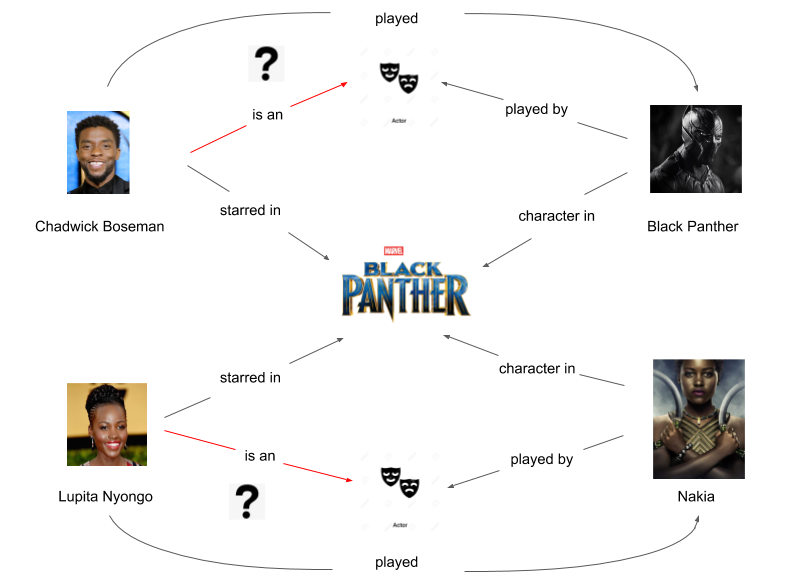
\includegraphics[width=0.8\textwidth, height=0.4\textheight]{Entities_and_the_Relationships_Between_Them}
	\captionsetup{justification=centering}
	\caption{Objects and relationships between them. We see Chadwick Boseman starred in the Black Panther film and played the Black Panther character. We also see that the character was played by an actor, and can reason that Chadwick Boseman may thus be an actor.}
\end{figure}

\subsection{Challenges} 

Reasoning about knowledge expressed in natural language \unskip~\citep{minervini2019differentiable} is simple for humans, but trying to imitate this behaviour on a computer reveals its underlying complexity. \par

\noindent The first task is providing a mechanism for perceiving syntax.\ Humans recognise text as sequences of words, and words as a sequence of characters. Characters can belong to different writing systems which can be dense (have a few characters used in a large number of combinations), or sparse (have a large number of characters used in fewer combinations) \unskip~\citep{Hua2010}. A computer has to first be able to perceive these characters. \par

\noindent The second task is even more challenging: modelling semantics. Semantics is the meaning of words in language \unskip~\citep{chomsky1955logical}. It allows humans to understand each other in conversation, through written text, and through visual imagery. Semantics allows us to understand that an actor is a thing, and that things can have relationships with other things. Giving computers the capability of semantic understanding is challenging because of the unstructuredness of language. If a person is shown a word in the singular and a word in the plural, for example "film" and "films", a person will most likely understand that there is not much difference in meaning between the two words, while a computer may interpret them as having completely different meanings. Different words can also have similar meanings, for example "film" and "movie". Capturing this similarity once again challenging for machines. And finally the order in which words are seen can provide context, for example the word "star" has completely different meanings in "Chadwick Boseman is a movie star" and "Black Panther looked up into the night sky and saw a star". \par

\noindent The third challenging task is organising information in such a way as to be able to reason about the knowledge it conveys. Humans build mental models using default reasoning \unskip~\citep{reiter1980logic}, believing that most objects A have some relationship X with objects B, with a small number of exceptions. For example, we could believe that films (object A) have not won (relationship X) an Oscar (object B). We will believe this is true for any given movie, unless we are familiar enough with movie history to identify the exceptions.\ Formally, the default beliefs we hold are facts, and this process of reasoning allows us to infer new facts in the form of plausible relationships between objects. \par

\noindent In order to allow computers to use a similar method of reasoning, facts can be represented as graph-structured data.\ Such a representation is called a knowledge graph (KG) and models facts as entities (nodes) and the relations (edges) between them \unskip~\citep{nickel2015review}. The Resource Description formalism (RDF) is used to encode facts as triples in the form, subject-predicate-object, where the subject and object are entities, and the predicate is a relation between two entities \unskip~\citep{bizer2009dbpedia}. For example, a fact (triple) in an entertainment KG would be Black Panther (subject/entity) is a (predicate/relation) super hero (object/entity). \par

\noindent Question answering (QA) relies on knowledge discovery, the step-by-step deductive process used to infer possible facts given known facts.\ This is the process used above to infer that Chadwick Boseman is an actor, given other facts known about Chadwick Boseman and the Black Panther film. Statistical relational learning (SRL) solves the knowledge discovery problem by constructing models with measures of uncertainty in plausible facts not contained in KGs \unskip~\citep{koller2007introduction}.\par

\subsection{Encouraging progress} 

The task of QA can be extended to an open-domain setting \unskip~\citep{chen2017reading}, where the task is extended from answering questions from a single domain to a multiple domains.\ In this setting, a KG contains data from multiple domains and more complex knowledge discovery chains be constructed. There has been encouraging progress in SRL to modelling this problem, and link prediction, inferring a plausible edge (relationship) between two KG nodes (entities), is now often used as a paradigm for knowledge discovery \unskip~\citep{kristiadi2019incorporating, ebisu2018toruse, nguyen2017novel}. Latent feature modelling using tensor factorisation \unskip~\citep{harshman1978models, kolda2009tensor} is an approach to link prediction that has seen some promising results \unskip~\citep{bordes2011learning, jenatton2012latent, nickel2016holographic}. \par 

\noindent The first major milestone was demonstrating the bilinear tensor product as a promising model to link prediction \unskip~\citep{nickel2011three}. In this model, the multiplication is taken between a subject vector and a predicate matrix, producing a entity-relational vector. The dot product is then taken between the entity-relational vector and an object vector, which generates a relational score between the subject and object entities. \par

\noindent The second milestone was the integration of the bilinear tensor product and neural networks \unskip~\citep{socher2013reasoning}. In this approach a recursive network \unskip~\citep{pollack1990recursive} computes a compositional score between the subject and object, which is then added to a bilinear tensor product score. The result is then passed through a nonlinearity which generates the final relational score. This approach effectively extended linear tensor factorisation techniques to nonlinear techniques, and simultaneously introduced the use of pre-trained word embeddings to initialise entity and relation vectors instead of random initialisation. In this one approach both decision making expressiveness as well as entity and relation semantic representations were improved. \par

\noindent The third time a milestone was realised was with the use of complex valued embeddings for link prediction \unskip~\citep{trouillon2016complex}. This approach extended the bilinear tensor product by making use of the Hermitian dot product, which is the complex counterpart of the standard dot product between real vectors. It was proposed that complex vectors can effectively capture antisymmetric relations, "is not", while retaining the efficiency benefits of the dot product. This was achieved by using representations with complex embeddings, allowing the model to capture semantic meaning by computing a relational score dependent on the order of the entities in the triple. \par
 
\noindent The above three milestones relied on shallow models that could scale to large datasets. Up until that point research in link prediction had focused on minimising the parameterisation of models. Convolutional networks are parameter efficient models, and major progress was again realised with the use of deep convolutional models for link prediction \unskip~\citep{dettmers2018convolutional}. The approach made use of 2D embedding representations which allowed the modelling of a large number of interactions between entities, achieving state-of-the-art (SOTA) link prediction performance as a result. \par

\subsection{Remaining challenges}

\noindent Open-domain knowledge graph question answering (KGQA) is getting closer to realising a form of AI reasoning generalisation. One significant challenge still faced by this framework is automatic construction of KGs \unskip~\citep{dong2014knowledge}. These large data sources are required to adequately train link prediction models. Combining such data sources for sufficient knowledge density remains an open area of research \unskip~\citep{diefenbach2018wdaqua}. Relying on systems with a graph structure alone limit the set of available resources which can be used to acquire knowledge \unskip~\citep{chen2017reading}, which necessitates the use of other source types including news document sets amongst others. Presenting this information poses a significant data transformation challenge, as well as potentially requiring continual online learning of the model as new data becomes available \unskip~\citep{abujabal2018never}. \par

\noindent It is also currently unclear which link prediction paradigm is the most useful in knowledge discovery. In addition to latent feature modelling, graph modelling \unskip~\citep{niepert2016discriminative, schlichtkrull2018modeling, pinter2018predicting} and inductive probabilistic logic programming (PLP) \unskip~\citep{speichert2018learning} are two approaches also used for link prediction. Graph modelling is a generalisation of latent feature modelling which aggregates local and global entity neighbourhood context to generate relational scores between entities. Inductive PLP introduces stochastic primitives to logic programming languages. Recently graph modelling has been receiving increased attention as an approach to link prediction, and may reveal efficient knowledge discovery patterns. \par

\noindent Finally, there seems to be large headroom for improvement in latent feature modelling based link prediction. SOTA performance on standard benchmark datasets, where the task of discovering the top 10 most plausible facts given an entity-relational composition, is currently achieved by a graph modelling technique \unskip~\citep{ruderNLPProg}. There is currently no human-level benchmark with which to contrast this performance, and it is also unclear whether improvement in link prediction performance can be realised by further optimisations to tensor factorisation approaches, or if a paradigm shift to graph modelling or inductive PLP will be required.  

\subsection{Outline of contributions}

We begin by introducing training algorithm optimisations to a TensorFlow \unskip~\citep{abadi2016tensorflow} reimplementation of the NTN model \unskip~\citep{Doss2015}.  We apply early stopping \unskip~\citep{prechelt1998early}, a regularisation technique that prevents overfitting of training data. We aslo apply adaptive moment estimation (Adam)  \unskip~\citep{kingma2014adam}, a parameter optimisation technique that makes use of an adaptive learning rate, where the learning rate is computed using the first and second order moments of the gradient. We also make use of random search hyperparamter optimisation \unskip~\citep{bergstra2012random} to tune the model. \par

\noindent HypER \unskip~\citep{balazevic2019hypernetwork} is a neural tensor factorisation model \unskip~\citep{wu2018neural} that introduces hypernetworks \unskip~\citep{ha2016hypernetworks} to latent feature modelling based link prediction. Hypernetworks are a class of meta neural networks used to generate a mapping from original inputs to hyper inputs, which are subsequently used in the forward pass of a main network. HypER uses a multilayer perceptron to transform relational vectors into relation-specific convolutional filters used by the main network. This hypernetwork suffers from covariate shift \unskip~\citep{ioffe2015batch}, the change in the distribution outputs from the previous layer in a network used as inputs to the current layer, caused by the simultaneous update of current and previous layer weights during back propagation. Covariate shift slows down training and degrades model performance during inference. We optimise the HypER training algorithm by applying batch normalisation, which compensates for covariate shift, and introduce HypER+. \par

\noindent Language models \unskip~\citep{turian2010word} are neural networks trained using very large text corpora. These models build a structural understanding of the syntax and semantics of a language, and are used to obtain pre-trained word vectors \unskip~\citep{mikolov2013distributed} for downstream tasks.\ Leveraging semantic information \unskip~\citep{socher2013reasoning} from pre-trained word vectors can provide richer latent representations for entities and relations, which may improve inference during knowledge discovery. We thus integrate pre-trained word vectors into the HypER+ training algorithm and use them to initialise entity and relational vectors in place of Xavier initialisation \unskip~\citep{glorot2010understanding}. 

\subsection{Long-term motivations} 

Imitation of human-level intelligence persists as an inspirational challenge to science. This challenge gave rise to the first attempts at AI research beginning with the perceptron \unskip~\citep{rosenblatt1958perceptron}, and continues to inspire the fervour present today. Intelligent virtual assistants like Ironman's J.A.R.V.I.S. (Just A Rather Very Intelligent System) \unskip~\citep{jarvisIronmanWiki}, serve as a North Star for the desired capabilities of natural language based AI systems. These systems can be thought of as artificial general intelligence (AGI), indistinguishable from human capabilities in reasoning, dialogue and humor. Possible applications of such a technology are numerous, where perhaps one of the most useful may be an AI tutoring interface for education. South Africa experiences many educational challenges, and such a system could have a profound impact in helping students.\ Open-domain question answering becomes particularly important in this setting, where practical implementations may be grounded in continuous online training of knowledge discovery models. This thesis explores ideas that aim to contribute incremental progress toward AGI.  

\subsection{Short-term motivations}

One of the challenges facing KGQA is the there exists no standard benchmark of human-level performance in knowledge discovery. Such a benchmark could be used to more qualitatively assess link prediction performance of existing approaches. The current SOTA link prediction model's performance may be consistent with the minimum level of performance required to sufficiently satisfy user questions, however until baseline metrics exist with which to measure this, it may remain difficult to quantitaviley validate gains in performance. \par

\noindent The most appropriate paradigm for knowledge discovery is also still an open question. Graph modelling has the advantage of longer sequences with which to build dependencies between entities. Such an advantage allows the modelling of relational correlations between entities that is not possible in latent feature modelling. Latent feature modelling has the advantage of computational efficiency. No matter how large the KG, latent feature modelling approaches remain adept at handling this density. Both of these paradigms are stochastic however, and in certain scenerios more determinstic approaches may be required, a strength of IPLP. Explainability of logic rules with stochastic primitives \unskip~\citep{yang2017differentiable} may useful in safety-critical applications, or under decision-making understanding contexts. \par

\noindent Knowledge discovery is currently fulfilled through the task of prediction.\ Two frameworks have been used to structure approaches to this task, probabilistic modelling and mathematical estimation of generative distributions (machine learning). Both of these frameworks rely on in-depth a priori structuring of a paradigm used as an approach to prediction, for example Bayesian inference, shallow models and deep models \unskip~\citep{murphy2012machine}. Each paradigm has given rise to a number of models and corresponding training algorithms with inherent strengths and weaknesses. The trend in prediction research however is simple models of ever increasing size, trained on very very large datasets.\ It is unclear whether careful curation of model definitions and training algorithms will be able to continue to compete with this more brute force alternative. Exploring the dissymmetric opposition of these two philosophies should guide the development of the most efficient solutions.

\subsection{Challenges of latent feature modelling} 

Tensor factorisation is the most common approach for latent feature modelling based link prediction.\ This model has a number of attractive properties including simplicity, efficient handling of sparse and high dimensional data, as well as compute efficiency. Extensions to linear tensor factorisation approaches have involved integration with deep models. This approach has been effective in improving performance, however recent results suggest there are higher levels to be achieved. Deep models typically contain a large number of parameters, and as a result are prone to poor link prediction generalisation. Training algorithm optimisations, specifically regarding regularisation, have proved useful in improving model generalisation. Increasing model complexity, whilst preserving test set generalisation continues to be a challenge. \par

\noindent Until recently, entity-relational interaction modelling has posed a significant challenge. Expressing a variety of dyadic interactions (e.g. antisymmetry) between entities, as well modellling KG nodes with high in degree has proved problematic. The use of nonlinear factorisation models has improved interaction representation. Determining model operators which extend expressiveness in interaction modelling may be useful in further improving performance.\par

\noindent Generating entity and relation representations is another challenge. Previous work represented entities and relations using randomly initialised, static embeddings. This approach does not allow the sharing of statistical strength between the embeddings describing each entity or relation. Chen et al. \unskip~\citep{socher2013reasoning} showed that using pre-trained word vectors instead of randomly initialised word embeddings improves link prediction performance. This performance gain can be explained by the co-occurrence statistics used to train word vectors. Language models \unskip~\citep{ bojanowski2016enriching, vaswani2017attention} may be useful in obtaining meaningful semantic representations for entity and relation vectors. They may also be useful in compensating for sparsity in interaction observations. \par

\noindent Compute resources required to perform inference also present a challenge.\ For any given entity-relational input pair, current methods compute a relation prediction score for every entity within the KG. This is not a challenge for KGs with a small number of entities (thousands), however poses a scalability problem for KGs with a large number entities (millions). Compute requirements thus continue to place a parameterisation constraint on latent feature models. 


%********************************** %Second Section  *************************************

\section{Related work} %Section - 1.2 

\subsection{Reasoning about facts} 

\noindent This thesis aims to extend research that aspires to give machines the capability of human-like reasoning \unskip~\citep{bordes2011learning} in open-domain question answering \unskip~\citep{hakimov2019evaluating}. Early work in this area focused on using relational data to learn deterministic logical rules based on symbolic representations, which were used for formal reasoning \unskip~\citep{hohenecker2017deep}.\ This approach gave rise to the inductive logic programming (ILP) paradigm, however due to finite domain utility, scalability issues and poor performance, research in reasoning shifted to statistical methods focused on attribute representation, which were increasingly successful in prediction tasks, particularly in computer vision and natural language processing (NLP) \unskip~\citep{koller2007introduction}.\ SRL is the hybridisation of these two approaches, learning statistical correlations between concept dependencies by leveraging structural information in relational data. \par

\noindent SRL is comprised of three paradigms, latent feature modelling, graph modelling and tensor factorisation \unskip~\citep{nickel2015review}. The rest of this dissertation is concerned with the analysis of approaches to latent feature modelling. Tensor factorisation has become one of the most popular approaches to latent feature modelling, where a decomposition of relational data represented as a tensor, is used to generate a set of constituent vectors, see Figure 1.2, and Figure 1.3. \par

\begin{figure}[H]
   	\centering
    	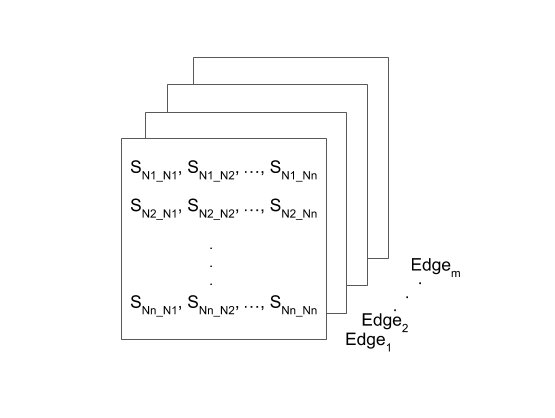
\includegraphics[width=0.6\textwidth, height=0.3\textheight]{relational_tensor.png}
	\captionsetup{justification=centering}
	\caption{Knowledge graph structured data represented as a relational tensor of size $ n \; x \; n \; x \; m $ with relational scores $ S $ between nodes, indexed by $ Edge $. $ S_{N1\_N2} $ is the relational score between node $ N1 $ and node $ N2 $ for $ Edge_1 $, in the range $ \in (0, 1] $. If an edge is present between these two nodes in the data, the score is $ 1.0 $.}
\end{figure}

\begin{figure}[H]
   	\centering
    	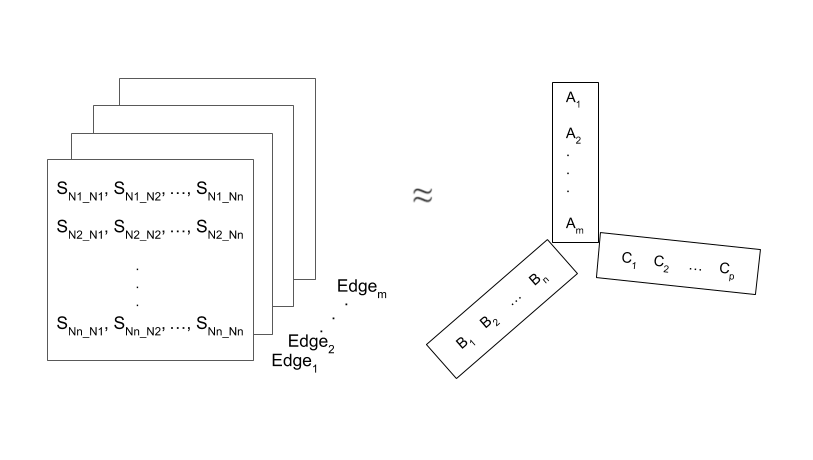
\includegraphics[width=0.7\textwidth, height=0.4\textwidth]{relational_tensor_decomposition}
	\captionsetup{justification=centering}
	\caption{Relational tensor decomposition into $ 3 $ constituent vectors $ A $, $ B $ and $ C $, where $ A \in \mathbb{R}^m $,  $ B \in \mathbb{R}^n $ and $ C \in \mathbb{R}^p $. The inner product of these vectors computes the relational tensor.}
\end{figure}

\noindent RESCAL, by Nickel et al.  \unskip~\citep{nickel2011three}, decomposes a relational tensor $ T_k $ into an entity matrix $ E  \in \mathbb{R}^{n x r} $, a set of relational matrices $ R_k \in \mathbb{R}^{rxr}$. The bilinear tensor product is the inner product between $ E $ and a slice $ k $ of $ R_k $, where the inner product of the result is taken with a transposed matrix $ E^T \in \mathbb{R}^{r x n} $, see equation 1.1.

\begin{equation}
	T_k \approx ER_kE^T
\end{equation}

\noindent Entity matrix $ E $ is composed of entity vectors $ e \in \mathbb{R}^r $ and a relation matrix $ k $ of the relational tensor $ R_k $ is represented as a full rank matrix $ W_k \in \mathbb{R}^{rxr} $ \unskip~\citep{nickel2012factorizing}.\ An inner product between an entity $ e_i $ and relational matrix $ W_k $, followed by an inner product with entity vector $ e_j $ generates a relational score $ n_{i,j,k} $. When adopting the RDF formalism, $ e_i $ is the subject, $ W_k $ is the predicate, and $ e_j $ is the object.\ This set comprises an RDF triple, used to encode a KG fact.\ Entities $ e_i $, and $ e_j $ and relation $ W_k $ have unknown latent representations, and the task is to learn the most optimal representations that can be used for relation prediction. The training algorithm minimises the squared error loss, and the model achieves competitive performance on various datasets. \par

\noindent Translating the embeddings (TransE) of entities is another model for relation prediction \unskip~\citep{bordes2013translating}. The motivation for this approach is that a lot of KG facts are presented in hierarchies, therefore a translation of the subject by the predicate should produce an embedding close to the object. The model translation is thus the natural transformation of the entity and can be used to model hierarchies, as well as modelling embedding equivalence with reverse transformations. \par

\noindent Yang et al. \unskip~\citep{yang2014embedding} proposed DistMult, a bilinear diagonal model which first transforms the subject and object entities into low-dimensional vector representations, and then applies a bilinear tensor product operation using a predicate matrix with only diagonal elements. This approach effectively models a subset of the entity-relational interactions of RESCAL, and relies on the entity transformations to generate sufficient semantic information. The model's bilinear formulation is extremely parameter efficient but lacks expressiveness. \par

\noindent ComplEx, by Trouillon et al. \unskip~\citep{trouillon2016complex}, is the extension of DistMult into the complex domain. Entities are represented using complex vectors, and relations are represented using a diagonal matrix with complex entries.\ Complex valued embeddings extend the modelling of entity-relational interactions to include antisymmetric interactions. \par

\noindent All these approaches rely on linear tensor factorisation for latent feature modelling, and aside from ComplEx, apply simple inner product operators for entity-relational interaction modelling. These representations scale well with large datasets but are limited in their expressiveness. Next we will discuss nonlinear models. \par

\noindent Neural tensor networks (NTN), by Chen et al. \unskip~\citep{socher2013reasoning}, extend the bilinear tensor product in two ways.\ Firstly, they make use of a recursive network (RCN) \unskip~\citep{socher2012semantic} to construct a composition between two entities and output a compositional score.\ This compositional score is then added to the output of the bilinear tensor product, generating a relational score. Secondly, the computed relational score is passed through a nonlinearity. The NTN achieves a higher level of relational expressiveness, significantly increasing relation prediction performance.  Chen et al. \unskip~\citep{socher2013reasoning} also assess the use of pre-trained word vectors on link prediction. They find pre-trained word vectors outperform random initialisation. \par

\noindent Hohenecker and Lukasiewicz \unskip~\citep{hohenecker2017deep} extend NTNs by pre-computing an object representation as an aggregation of all facts (triples) in which the object plays a part.\ They introduce the new model as a relational NTN (RTN). Dong et al. \unskip~\citep{dong2014knowledge} introduced ER-MLP, a two layer multilayer perceptron (MLP) which takes a triple as an input set of vectors, and passes this input to a fully-connected layer. The layer generates a hidden output vector which is passed through a nonlinearity, and finally through a second fully-connected layer.\ ER-MLP makes use of low-dimensional vectors for embedding representations. \par

\noindent HolE, Nickel et al. \unskip~\citep{nickel2016holographic}, uses a circular correlation as an operator during relation prediction. The multiplication between subject $ s $ and object $ o $ features is taken by sliding the object over the subject, see equations 1.2a, 1.2b and 1.2c. 
\begin{subequations}
	\begin{gather}
		c_0 =  (s_0*o_0 + s_1*o_1 + s_2*o_2) \\
		c_1 =  (s_0*o_2 + s_1*o_0 + s_2*o_1) \\
		c_2 =  (s_0*o_1 + s_1*o_2 + s_2*o_0) 
	\end{gather}
\end{subequations}

\noindent where $ c_0, \; c_1, \; c_2 $ are items of a correlation vector.\ An inner product is then taken with a predicate vector which generates a relational score.\ HolE is particularly adept at modelling antisymmetric interactions. \par

\noindent ConvE, Dettmers et al.  \unskip~\citep{dettmers2018convolutional}, introduces the use of the convolutional operator in entity-relational modelling. The model lengthwise concatenates the subject vector $ S \in \mathbb{R}^{k} $ with itself, and then lengthwise concatenates a predicate vector $ P \in \mathbb{R}^{k} $ with itself, creating two matrices $ S \in \mathbb{R}^{2k} $ and $ P \in \mathbb{R}^{2k} $, where $ k $  is the vector length. $ S $ and $ P $ are then lengthwise concatenated to create an entity-relational matrix $ M \in \mathbb{R}^{4k} $, see equations 1.3.
\begin{equation}
	(\begin{bmatrix}
        		s & s & s \\
           	s & s & s 
       	\end{bmatrix}); \; (\begin{bmatrix}
        					p & p & p \\
           				p & p & p 
       				\end{bmatrix}) = \begin{bmatrix}
        								s & s & s \\
           							s & s & s \\
           							p & p & p \\
           							p & p & p
        			     				\end{bmatrix}
\end{equation}

\noindent A convolution is then performed on the $ M $ using a convolutional filter. The same filter is used for convolutions across all subject-predicate combinations, allowing for parameter sharing across triples. The convolution generates a feature map which is passed to a fully-connected layer that flattens it into an entity-relational hidden vector. Finally, the inner product of the hidden vector is taken with all object vectors, which generates a relational score for each object. The convolutional operator increases expressiveness by modelling entity-relational interactions around the entire concatenation line, enabling high levels of relation prediction performance. \par

\noindent The above approaches comprise nonlinear tensor factorisation for latent feature modelling. And all, excluding HolE, introduce neural tensor factorisation.\ Two other paradigms, graph modelling and IPLP, apply alternative approaches to link prediction.\ We refer the reader to \unskip~\citep{nickel2015review} for a recent review. \par


%********************************** % Third Section  *************************************

\section{Contributions and outline} %Section - 1.3

\noindent In this thesis we explore neural tensor factorisation models used for latent feature modelling in link prediction.\ We assess how nonlinear extensions of the bilinear tensor product, and the use of convolutional operators for entity-relational modelling, result in higher levels of expressiveness. In particular, we attempt to further improve model performance by optimising the training algorithm, with particular attention to regularisation. To this end, we update the NTN training algorithm with modern regularisation, optimisation and hyperparameter tuning techniques.\ We then compensate for covariate shift introduced by hypernetworks, and use pre-trained word vectors for embedding in initialisation. \par

\noindent In \textbf{Chapter 2} we discuss training algorithm approaches based on the supervised learning paradigm. We then discuss deep learning models, specifically in relation to convolutional and recurrent networks.\ We provide mathematical definitions for the models, and discuss the primary problems they aim to address, as well as examples of applications.\ We present regularisation techniques used to address overfitting, where we explore early stopping \unskip~\citep{prechelt1998early}, dropout \unskip ~\citep{srivastava2014dropout} and batch normalisation \unskip ~\citep{ioffe2015batch}. Finally we discuss language models \unskip~\citep{ bojanowski2016enriching, vaswani2017attention} and their utility in semantic representations. \par

\noindent In \textbf{Chapter 3} we begin by exploring the NTN model introduced by Chen et al. \unskip ~\citep{socher2013reasoning} and reimplemented in TensorFlow by Doss et al. \unskip ~\citep{Doss2015}.\ We assess the expressive strengths of this model due to the addition of entity-compositional modelling using an RCN \unskip ~\citep{socher2012semantic}, and initialisation of word embeddings using pre-trained word vectors.\ We then explore reimplementing the model ourselves, and applying early stopping, Adam \unskip ~\citep{kingma2014adam} and hyperparameter random search \unskip ~\citep{bergstra2012random} to the training algorithm. \par

\noindent We continue with exploring the HypER model introduced by Bala\v{z}evi\'c et al. \unskip ~\citep{balazevic2019hypernetwork}.\ We assess the expressive strengths of this model due to making use of the hypernetwork architecture \unskip ~\citep{ha2016hypernetworks} to generate relation-specific convolutional filters. The convolution between these filters and entities are used to construct representations which are ultimately used for relation prediction. We explore compensating for covariate shift caused by hypernetworks, and apply batch normalisation, introducing HypER+. We then initialise HypER+ embeddings using GloVe \unskip~\citep{pennington2014glove} pre-trained word vectors. \par

\noindent In \textbf{Chapter 4} we conduct a number of experiments to test the hypotheses concerning the training algorithms of the respective models, derived in the previous chapter.\ We begin by discussing the WordNet \unskip ~\citep{miller1995wordnet} and Freebase \unskip ~\citep{bollacker2008freebase} link prediction benchmark datasets.\ We use them to establish baseline cost and accuracy performance metrics for the reimplimented NTN TensorFlow model. We train the reimplimented model using an updated training algorithm, and compare the performance against the baseline. \par

\noindent We then discuss the WN18 \unskip ~\citep{bordes2014semantic} and FB15k \unskip ~\citep{bordes2013translating} link prediction benchmark datasets, as well benchmark metrics used for those datasets.\ We train the HypER+ model on the updated HypER training algorithm, and compare the performance against the baseline. Finally we discuss the WN18RR \unskip ~\citep{dettmers2018convolutional} and FB15k-237 \unskip ~\citep{toutanova2015observed} link prediction benchmark datasets. We extend HypER+ to take advantage of GloVe pre-trained vectors, and  compare the performance first against the HypER baseline, and then against HypER+ without pre-trained word vectors. \par

\noindent In \textbf{Chapter 5} we summarise the thesis and identify opportunities for neural tensor factorisation. We comment on the suitability of latent feature modelling for link prediction, in contrast with alternative paradigms, and assess the current utility of KGQA. We conclude with proposals for future research.

